\documentclass[1p]{elsarticle_modified}
%\bibliographystyle{elsarticle-num}

%\usepackage[colorlinks]{hyperref}
%\usepackage{abbrmath_seonhwa} %\Abb, \Ascr, \Acal ,\Abf, \Afrak
\usepackage{amsfonts}
\usepackage{amssymb}
\usepackage{amsmath}
\usepackage{amsthm}
\usepackage{scalefnt}
\usepackage{amsbsy}
\usepackage{kotex}
\usepackage{caption}
\usepackage{subfig}
\usepackage{color}
\usepackage{graphicx}
\usepackage{xcolor} %% white, black, red, green, blue, cyan, magenta, yellow
\usepackage{float}
\usepackage{setspace}
\usepackage{hyperref}

\usepackage{tikz}
\usetikzlibrary{arrows}

\usepackage{multirow}
\usepackage{array} % fixed length table
\usepackage{hhline}

%%%%%%%%%%%%%%%%%%%%%
\makeatletter
\renewcommand*\env@matrix[1][\arraystretch]{%
	\edef\arraystretch{#1}%
	\hskip -\arraycolsep
	\let\@ifnextchar\new@ifnextchar
	\array{*\c@MaxMatrixCols c}}
\makeatother %https://tex.stackexchange.com/questions/14071/how-can-i-increase-the-line-spacing-in-a-matrix
%%%%%%%%%%%%%%%

\usepackage[normalem]{ulem}

\newcommand{\msout}[1]{\ifmmode\text{\sout{\ensuremath{#1}}}\else\sout{#1}\fi}
%SOURCE: \msout is \stkout macro in https://tex.stackexchange.com/questions/20609/strikeout-in-math-mode

\newcommand{\cancel}[1]{
	\ifmmode
	{\color{red}\msout{#1}}
	\else
	{\color{red}\sout{#1}}
	\fi
}

\newcommand{\add}[1]{
	{\color{blue}\uwave{#1}}
}

\newcommand{\replace}[2]{
	\ifmmode
	{\color{red}\msout{#1}}{\color{blue}\uwave{#2}}
	\else
	{\color{red}\sout{#1}}{\color{blue}\uwave{#2}}
	\fi
}

\newcommand{\Sol}{\mathcal{S}} %segment
\newcommand{\D}{D} %diagram
\newcommand{\A}{\mathcal{A}} %arc


%%%%%%%%%%%%%%%%%%%%%%%%%%%%%5 test

\def\sl{\operatorname{\textup{SL}}(2,\Cbb)}
\def\psl{\operatorname{\textup{PSL}}(2,\Cbb)}
\def\quan{\mkern 1mu \triangleright \mkern 1mu}

\theoremstyle{definition}
\newtheorem{thm}{Theorem}[section]
\newtheorem{prop}[thm]{Proposition}
\newtheorem{lem}[thm]{Lemma}
\newtheorem{ques}[thm]{Question}
\newtheorem{cor}[thm]{Corollary}
\newtheorem{defn}[thm]{Definition}
\newtheorem{exam}[thm]{Example}
\newtheorem{rmk}[thm]{Remark}
\newtheorem{alg}[thm]{Algorithm}

\newcommand{\I}{\sqrt{-1}}
\begin{document}

%\begin{frontmatter}
%
%\title{Boundary parabolic representations of knots up to 8 crossings}
%
%%% Group authors per affiliation:
%\author{Yunhi Cho} 
%\address{Department of Mathematics, University of Seoul, Seoul, Korea}
%\ead{yhcho@uos.ac.kr}
%
%
%\author{Seonhwa Kim} %\fnref{s_kim}}
%\address{Center for Geometry and Physics, Institute for Basic Science, Pohang, 37673, Korea}
%\ead{ryeona17@ibs.re.kr}
%
%\author{Hyuk Kim}
%\address{Department of Mathematical Sciences, Seoul National University, Seoul 08826, Korea}
%\ead{hyukkim@snu.ac.kr}
%
%\author{Seokbeom Yoon}
%\address{Department of Mathematical Sciences, Seoul National University, Seoul, 08826,  Korea}
%\ead{sbyoon15@snu.ac.kr}
%
%\begin{abstract}
%We find all boundary parabolic representation of knots up to 8 crossings.
%
%\end{abstract}
%\begin{keyword}
%    \MSC[2010] 57M25 
%\end{keyword}
%
%\end{frontmatter}

%\linenumbers
%\tableofcontents
%
\newcommand\colored[1]{\textcolor{white}{\rule[-0.35ex]{0.8em}{1.4ex}}\kern-0.8em\color{red} #1}%
%\newcommand\colored[1]{\textcolor{white}{ #1}\kern-2.17ex	\textcolor{white}{ #1}\kern-1.81ex	\textcolor{white}{ #1}\kern-2.15ex\color{red}#1	}

{\Large $\underline{11a_{126}~(K11a_{126})}$}

\setlength{\tabcolsep}{10pt}
\renewcommand{\arraystretch}{1.6}
\vspace{1cm}\begin{tabular}{m{100pt}>{\centering\arraybackslash}m{274pt}}
\multirow{5}{120pt}{
	\centering
	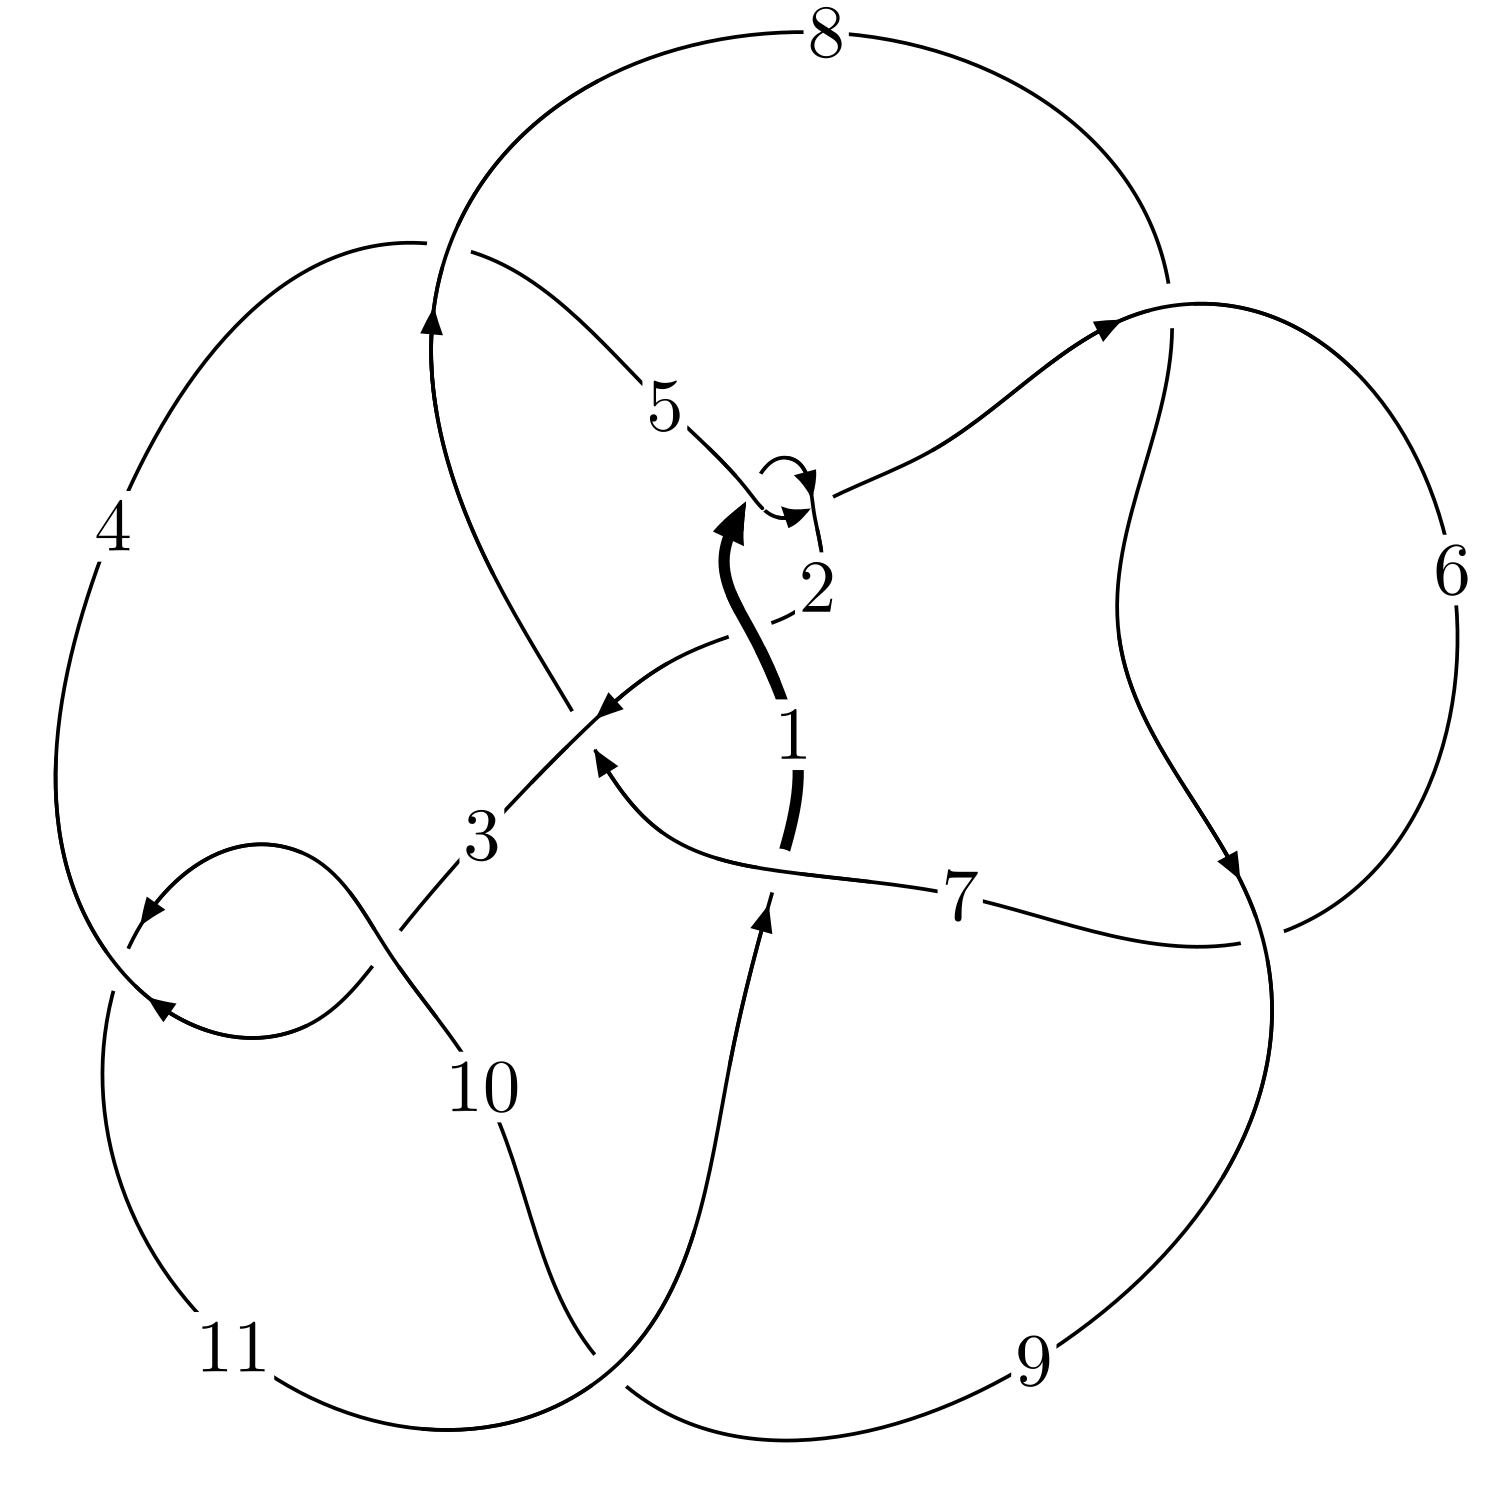
\includegraphics[width=112pt]{../../../GIT/diagram.site/Diagrams/png/375_11a_126.png}\\
\ \ \ A knot diagram\footnotemark}&
\allowdisplaybreaks
\textbf{Linearized knot diagam} \\
\cline{2-2}
 &
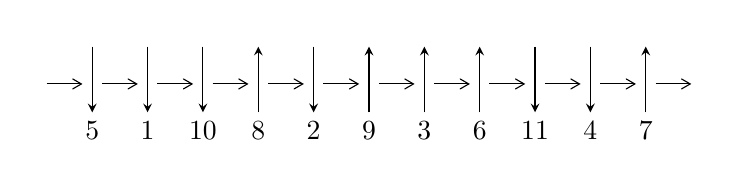
\begin{tikzpicture}[x=20pt, y=17pt]
	% nodes
	\node (C0) at (0, 0) {};
	\node (C1) at (1, 0) {};
	\node (C1U) at (1, +1) {};
	\node (C1D) at (1, -1) {5};

	\node (C2) at (2, 0) {};
	\node (C2U) at (2, +1) {};
	\node (C2D) at (2, -1) {1};

	\node (C3) at (3, 0) {};
	\node (C3U) at (3, +1) {};
	\node (C3D) at (3, -1) {10};

	\node (C4) at (4, 0) {};
	\node (C4U) at (4, +1) {};
	\node (C4D) at (4, -1) {8};

	\node (C5) at (5, 0) {};
	\node (C5U) at (5, +1) {};
	\node (C5D) at (5, -1) {2};

	\node (C6) at (6, 0) {};
	\node (C6U) at (6, +1) {};
	\node (C6D) at (6, -1) {9};

	\node (C7) at (7, 0) {};
	\node (C7U) at (7, +1) {};
	\node (C7D) at (7, -1) {3};

	\node (C8) at (8, 0) {};
	\node (C8U) at (8, +1) {};
	\node (C8D) at (8, -1) {6};

	\node (C9) at (9, 0) {};
	\node (C9U) at (9, +1) {};
	\node (C9D) at (9, -1) {11};

	\node (C10) at (10, 0) {};
	\node (C10U) at (10, +1) {};
	\node (C10D) at (10, -1) {4};

	\node (C11) at (11, 0) {};
	\node (C11U) at (11, +1) {};
	\node (C11D) at (11, -1) {7};
	\node (C12) at (12, 0) {};

	% arrows
	\draw[->,>={angle 60}]
	(C0) edge (C1) (C1) edge (C2) (C2) edge (C3) (C3) edge (C4) (C4) edge (C5) (C5) edge (C6) (C6) edge (C7) (C7) edge (C8) (C8) edge (C9) (C9) edge (C10) (C10) edge (C11) (C11) edge (C12) ;	\draw[->,>=stealth]
	(C1U) edge (C1D) (C2U) edge (C2D) (C3U) edge (C3D) (C4D) edge (C4U) (C5U) edge (C5D) (C6D) edge (C6U) (C7D) edge (C7U) (C8D) edge (C8U) (C9U) edge (C9D) (C10U) edge (C10D) (C11D) edge (C11U) ;
	\end{tikzpicture} \\
\hhline{~~} \\& 
\textbf{Solving Sequence} \\ \cline{2-2} 
 &
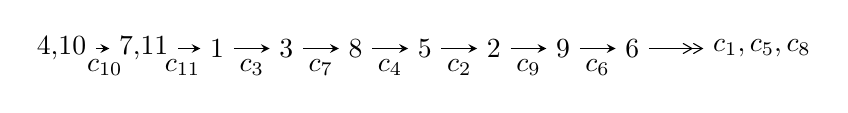
\begin{tikzpicture}[x=25pt, y=7pt]
	% node
	\node (A0) at (-1/8, 0) {4,10};
	\node (A1) at (17/16, 0) {7,11};
	\node (A2) at (17/8, 0) {1};
	\node (A3) at (25/8, 0) {3};
	\node (A4) at (33/8, 0) {8};
	\node (A5) at (41/8, 0) {5};
	\node (A6) at (49/8, 0) {2};
	\node (A7) at (57/8, 0) {9};
	\node (A8) at (65/8, 0) {6};
	\node (C1) at (1/2, -1) {$c_{10}$};
	\node (C2) at (13/8, -1) {$c_{11}$};
	\node (C3) at (21/8, -1) {$c_{3}$};
	\node (C4) at (29/8, -1) {$c_{7}$};
	\node (C5) at (37/8, -1) {$c_{4}$};
	\node (C6) at (45/8, -1) {$c_{2}$};
	\node (C7) at (53/8, -1) {$c_{9}$};
	\node (C8) at (61/8, -1) {$c_{6}$};
	\node (A9) at (10, 0) {$c_{1},c_{5},c_{8}$};

	% edge
	\draw[->,>=stealth]	
	(A0) edge (A1) (A1) edge (A2) (A2) edge (A3) (A3) edge (A4) (A4) edge (A5) (A5) edge (A6) (A6) edge (A7) (A7) edge (A8) ;
	\draw[->>,>={angle 60}]	
	(A8) edge (A9);
\end{tikzpicture} \\ 

\end{tabular} \\

\footnotetext{
The image of knot diagram is generated by the software ``\textbf{Draw programme}" developed by Andrew Bartholomew(\url{http://www.layer8.co.uk/maths/draw/index.htm\#Running-draw}), where we modified some parts for our purpose(\url{https://github.com/CATsTAILs/LinksPainter}).
}\phantom \\ \newline 
\centering \textbf{Ideals for irreducible components\footnotemark of $X_{\text{par}}$} 
 
\begin{align*}
I^u_{1}&=\langle 
-3 u^{17}+2 u^{16}+\cdots+8 b-8,\;-7 u^{17}-2 u^{16}+\cdots+8 a-20,\;u^{18}+u^{17}+\cdots+3 u+1\rangle \\
I^u_{2}&=\langle 
-2.20753\times10^{40} u^{55}+6.11690\times10^{40} u^{54}+\cdots+4.92510\times10^{40} b-2.71302\times10^{40},\\
\phantom{I^u_{2}}&\phantom{= \langle  }1.18198\times10^{40} u^{55}-2.66851\times10^{40} u^{54}+\cdots+4.92510\times10^{40} a-1.69808\times10^{41},\;u^{56}-3 u^{55}+\cdots-2 u+1\rangle \\
I^u_{3}&=\langle 
2 b- u-2,\;2 a- u-2,\;u^2+u-1\rangle \\
\\
\end{align*}
\raggedright * 3 irreducible components of $\dim_{\mathbb{C}}=0$, with total 76 representations.\\
\footnotetext{All coefficients of polynomials are rational numbers. But the coefficients are sometimes approximated in decimal forms when there is not enough margin.}
\newpage
\renewcommand{\arraystretch}{1}
\centering \section*{I. $I^u_{1}= \langle -3 u^{17}+2 u^{16}+\cdots+8 b-8,\;-7 u^{17}-2 u^{16}+\cdots+8 a-20,\;u^{18}+u^{17}+\cdots+3 u+1 \rangle$}
\flushleft \textbf{(i) Arc colorings}\\
\begin{tabular}{m{7pt} m{180pt} m{7pt} m{180pt} }
\flushright $a_{4}=$&$\begin{pmatrix}0\\u\end{pmatrix}$ \\
\flushright $a_{10}=$&$\begin{pmatrix}1\\0\end{pmatrix}$ \\
\flushright $a_{7}=$&$\begin{pmatrix}\frac{7}{8} u^{17}+\frac{1}{4} u^{16}+\cdots-\frac{15}{8} u+\frac{5}{2}\\\frac{3}{8} u^{17}-\frac{1}{4} u^{16}+\cdots-\frac{3}{8} u+1\end{pmatrix}$ \\
\flushright $a_{11}=$&$\begin{pmatrix}1\\u^2\end{pmatrix}$ \\
\flushright $a_{1}=$&$\begin{pmatrix}-\frac{1}{2} u^{17}-\frac{3}{16} u^{16}+\cdots+\frac{7}{8} u-\frac{13}{16}\\-\frac{1}{2} u^{17}-\frac{3}{16} u^{16}+\cdots-\frac{1}{8} u-\frac{13}{16}\end{pmatrix}$ \\
\flushright $a_{3}=$&$\begin{pmatrix}u\\u\end{pmatrix}$ \\
\flushright $a_{8}=$&$\begin{pmatrix}\frac{3}{8} u^{17}+\frac{1}{4} u^{16}+\cdots-\frac{11}{8} u+\frac{5}{2}\\-\frac{1}{8} u^{17}-\frac{1}{4} u^{16}+\cdots+\frac{1}{8} u+1\end{pmatrix}$ \\
\flushright $a_{5}=$&$\begin{pmatrix}-\frac{1}{2} u^{17}-\frac{3}{16} u^{16}+\cdots+\frac{7}{8} u-\frac{29}{16}\\-\frac{1}{2} u^{17}-\frac{3}{16} u^{16}+\cdots+\frac{7}{8} u-\frac{13}{16}\end{pmatrix}$ \\
\flushright $a_{2}=$&$\begin{pmatrix}-0.187500 u^{17}-0.0625000 u^{16}+\cdots+0.562500 u-0.312500\\-0.187500 u^{17}-0.0625000 u^{16}+\cdots+0.562500 u-0.312500\end{pmatrix}$ \\
\flushright $a_{9}=$&$\begin{pmatrix}- u^2+1\\- u^4\end{pmatrix}$ \\
\flushright $a_{6}=$&$\begin{pmatrix}\frac{5}{8} u^{17}+\frac{1}{4} u^{16}+\cdots-\frac{5}{8} u+2\\\frac{5}{8} u^{17}+\frac{1}{4} u^{16}+\cdots-\frac{5}{8} u+1\end{pmatrix}$\\ \flushright $a_{6}=$&$\begin{pmatrix}\frac{5}{8} u^{17}+\frac{1}{4} u^{16}+\cdots-\frac{5}{8} u+2\\\frac{5}{8} u^{17}+\frac{1}{4} u^{16}+\cdots-\frac{5}{8} u+1\end{pmatrix}$\\&\end{tabular}
\flushleft \textbf{(ii) Obstruction class $= -1$}\\~\\
\flushleft \textbf{(iii) Cusp Shapes $= \frac{37}{8} u^{17}+\frac{49}{16} u^{16}-19 u^{15}-\frac{161}{16} u^{14}+\frac{175}{4} u^{13}+\frac{625}{16} u^{12}-\frac{1021}{16} u^{11}-79 u^{10}+\frac{489}{8} u^9+\frac{1847}{16} u^8-\frac{101}{4} u^7-\frac{481}{4} u^6-\frac{63}{8} u^5+\frac{313}{4} u^4+\frac{403}{16} u^3-\frac{275}{8} u^2-\frac{77}{4} u+\frac{115}{16}$}\\~\\
\newpage\renewcommand{\arraystretch}{1}
\flushleft \textbf{(iv) u-Polynomials at the component}\newline \\
\begin{tabular}{m{50pt}|m{274pt}}
Crossings & \hspace{64pt}u-Polynomials at each crossing \\
\hline $$\begin{aligned}c_{1},c_{3},c_{5}\\c_{10}\end{aligned}$$&$\begin{aligned}
&u^{18}- u^{17}+\cdots-3 u+1
\end{aligned}$\\
\hline $$\begin{aligned}c_{2},c_{9}\end{aligned}$$&$\begin{aligned}
&u^{18}+9 u^{17}+\cdots+19 u+1
\end{aligned}$\\
\hline $$\begin{aligned}c_{4},c_{11}\end{aligned}$$&$\begin{aligned}
&4(4 u^{18}-2 u^{17}+\cdots-10 u^2+1)
\end{aligned}$\\
\hline $$\begin{aligned}c_{6},c_{8}\end{aligned}$$&$\begin{aligned}
&u^{18}- u^{17}+\cdots+24 u-16
\end{aligned}$\\
\hline $$\begin{aligned}c_{7}\end{aligned}$$&$\begin{aligned}
&u^{18}+5 u^{17}+\cdots-384 u-64
\end{aligned}$\\
\hline
\end{tabular}\\~\\
\newpage\renewcommand{\arraystretch}{1}
\flushleft \textbf{(v) Riley Polynomials at the component}\newline \\
\begin{tabular}{m{50pt}|m{274pt}}
Crossings & \hspace{64pt}Riley Polynomials at each crossing \\
\hline $$\begin{aligned}c_{1},c_{3},c_{5}\\c_{10}\end{aligned}$$&$\begin{aligned}
&y^{18}-9 y^{17}+\cdots-19 y+1
\end{aligned}$\\
\hline $$\begin{aligned}c_{2},c_{9}\end{aligned}$$&$\begin{aligned}
&y^{18}+3 y^{17}+\cdots-159 y+1
\end{aligned}$\\
\hline $$\begin{aligned}c_{4},c_{11}\end{aligned}$$&$\begin{aligned}
&16(16 y^{18}-140 y^{17}+\cdots-20 y+1)
\end{aligned}$\\
\hline $$\begin{aligned}c_{6},c_{8}\end{aligned}$$&$\begin{aligned}
&y^{18}-13 y^{17}+\cdots+736 y+256
\end{aligned}$\\
\hline $$\begin{aligned}c_{7}\end{aligned}$$&$\begin{aligned}
&y^{18}-3 y^{17}+\cdots-104960 y+4096
\end{aligned}$\\
\hline
\end{tabular}\\~\\
\newpage\flushleft \textbf{(vi) Complex Volumes and Cusp Shapes}
$$\begin{array}{c|c|c}  
\text{Solutions to }I^u_{1}& \I (\text{vol} + \sqrt{-1}CS) & \text{Cusp shape}\\
 \hline 
\begin{aligned}
u &= \phantom{-}0.797207 + 0.665416 I \\
a &= \phantom{-}1.148400 - 0.556457 I \\
b &= \phantom{-}1.65807 + 1.34345 I\end{aligned}
 & \phantom{-}5.71206 - 2.89420 I & \phantom{-}7.03507 + 3.97344 I \\ \hline\begin{aligned}
u &= \phantom{-}0.797207 - 0.665416 I \\
a &= \phantom{-}1.148400 + 0.556457 I \\
b &= \phantom{-}1.65807 - 1.34345 I\end{aligned}
 & \phantom{-}5.71206 + 2.89420 I & \phantom{-}7.03507 - 3.97344 I \\ \hline\begin{aligned}
u &= -0.544045 + 0.930838 I \\
a &= -1.159100 + 0.772519 I \\
b &= \phantom{-}0.041004 + 1.409830 I\end{aligned}
 & \phantom{-}8.53344 - 5.24003 I & \phantom{-}5.37319 + 1.81946 I \\ \hline\begin{aligned}
u &= -0.544045 - 0.930838 I \\
a &= -1.159100 - 0.772519 I \\
b &= \phantom{-}0.041004 - 1.409830 I\end{aligned}
 & \phantom{-}8.53344 + 5.24003 I & \phantom{-}5.37319 - 1.81946 I \\ \hline\begin{aligned}
u &= -0.615364 + 0.642798 I \\
a &= \phantom{-}1.64986 - 0.81674 I \\
b &= \phantom{-}0.16727 - 1.68913 I\end{aligned}
 & \phantom{-}2.54047 - 0.51745 I & \phantom{-}4.03732 + 0.45208 I \\ \hline\begin{aligned}
u &= -0.615364 - 0.642798 I \\
a &= \phantom{-}1.64986 + 0.81674 I \\
b &= \phantom{-}0.16727 + 1.68913 I\end{aligned}
 & \phantom{-}2.54047 + 0.51745 I & \phantom{-}4.03732 - 0.45208 I \\ \hline\begin{aligned}
u &= -0.910004 + 0.658534 I \\
a &= -1.06248 + 1.71896 I \\
b &= \phantom{-}0.86916 + 1.64057 I\end{aligned}
 & \phantom{-}5.01031 + 7.38290 I & \phantom{-}4.96124 - 9.00655 I \\ \hline\begin{aligned}
u &= -0.910004 - 0.658534 I \\
a &= -1.06248 - 1.71896 I \\
b &= \phantom{-}0.86916 - 1.64057 I\end{aligned}
 & \phantom{-}5.01031 - 7.38290 I & \phantom{-}4.96124 + 9.00655 I \\ \hline\begin{aligned}
u &= -1.122640 + 0.135484 I \\
a &= -0.185979 - 0.361024 I \\
b &= -0.351910 + 0.563133 I\end{aligned}
 & -6.23953 + 2.23591 I & -10.20911 - 3.70336 I \\ \hline\begin{aligned}
u &= -1.122640 - 0.135484 I \\
a &= -0.185979 + 0.361024 I \\
b &= -0.351910 - 0.563133 I\end{aligned}
 & -6.23953 - 2.23591 I & -10.20911 + 3.70336 I\\
 \hline 
 \end{array}$$\newpage$$\begin{array}{c|c|c}  
\text{Solutions to }I^u_{1}& \I (\text{vol} + \sqrt{-1}CS) & \text{Cusp shape}\\
 \hline 
\begin{aligned}
u &= \phantom{-}1.015940 + 0.632188 I \\
a &= -1.96168 - 0.59613 I \\
b &= -1.46082 - 2.17214 I\end{aligned}
 & \phantom{-}0.14328 - 10.60240 I & -0.95783 + 10.15251 I \\ \hline\begin{aligned}
u &= \phantom{-}1.015940 - 0.632188 I \\
a &= -1.96168 + 0.59613 I \\
b &= -1.46082 + 2.17214 I\end{aligned}
 & \phantom{-}0.14328 + 10.60240 I & -0.95783 - 10.15251 I \\ \hline\begin{aligned}
u &= \phantom{-}0.733103 + 0.109565 I \\
a &= \phantom{-}0.931581 + 0.476227 I \\
b &= \phantom{-}0.056089 + 0.202732 I\end{aligned}
 & -1.331030 - 0.143749 I & -7.24003 - 0.28764 I \\ \hline\begin{aligned}
u &= \phantom{-}0.733103 - 0.109565 I \\
a &= \phantom{-}0.931581 - 0.476227 I \\
b &= \phantom{-}0.056089 - 0.202732 I\end{aligned}
 & -1.331030 + 0.143749 I & -7.24003 + 0.28764 I \\ \hline\begin{aligned}
u &= \phantom{-}1.107060 + 0.702923 I \\
a &= \phantom{-}1.64797 + 0.90506 I \\
b &= \phantom{-}1.31912 + 2.15841 I\end{aligned}
 & \phantom{-}5.0646 - 17.2092 I & \phantom{-}0.64160 + 10.07684 I \\ \hline\begin{aligned}
u &= \phantom{-}1.107060 - 0.702923 I \\
a &= \phantom{-}1.64797 - 0.90506 I \\
b &= \phantom{-}1.31912 - 2.15841 I\end{aligned}
 & \phantom{-}5.0646 + 17.2092 I & \phantom{-}0.64160 - 10.07684 I \\ \hline\begin{aligned}
u &= -1.64128\phantom{ +0.000000I} \\
a &= -0.142074\phantom{ +0.000000I} \\
b &= -0.00357888\phantom{ +0.000000I}\end{aligned}
 & -7.18406\phantom{ +0.000000I} & \phantom{-}75.4440\phantom{ +0.000000I} \\ \hline\begin{aligned}
u &= -0.281225\phantom{ +0.000000I} \\
a &= \phantom{-}2.62494\phantom{ +0.000000I} \\
b &= \phantom{-}0.907601\phantom{ +0.000000I}\end{aligned}
 & \phantom{-}1.21562\phantom{ +0.000000I} & \phantom{-}9.77320\phantom{ +0.000000I}\\
 \hline 
 \end{array}$$\newpage\newpage\renewcommand{\arraystretch}{1}
\centering \section*{II. $I^u_{2}= \langle -2.21\times10^{40} u^{55}+6.12\times10^{40} u^{54}+\cdots+4.93\times10^{40} b-2.71\times10^{40},\;1.18\times10^{40} u^{55}-2.67\times10^{40} u^{54}+\cdots+4.93\times10^{40} a-1.70\times10^{41},\;u^{56}-3 u^{55}+\cdots-2 u+1 \rangle$}
\flushleft \textbf{(i) Arc colorings}\\
\begin{tabular}{m{7pt} m{180pt} m{7pt} m{180pt} }
\flushright $a_{4}=$&$\begin{pmatrix}0\\u\end{pmatrix}$ \\
\flushright $a_{10}=$&$\begin{pmatrix}1\\0\end{pmatrix}$ \\
\flushright $a_{7}=$&$\begin{pmatrix}-0.239991 u^{55}+0.541817 u^{54}+\cdots-0.125309 u+3.44782\\0.448220 u^{55}-1.24198 u^{54}+\cdots+1.17141 u+0.550856\end{pmatrix}$ \\
\flushright $a_{11}=$&$\begin{pmatrix}1\\u^2\end{pmatrix}$ \\
\flushright $a_{1}=$&$\begin{pmatrix}-0.465735 u^{55}-1.13841 u^{54}+\cdots-2.39038 u+0.0140502\\-1.87437 u^{55}+2.39826 u^{54}+\cdots-5.31879 u+2.17450\end{pmatrix}$ \\
\flushright $a_{3}=$&$\begin{pmatrix}u\\u\end{pmatrix}$ \\
\flushright $a_{8}=$&$\begin{pmatrix}-0.279271 u^{55}+0.501862 u^{54}+\cdots-0.251857 u+3.16698\\0.408940 u^{55}-1.28194 u^{54}+\cdots+1.04486 u+0.270025\end{pmatrix}$ \\
\flushright $a_{5}=$&$\begin{pmatrix}-1.72196 u^{55}+4.91727 u^{54}+\cdots+4.36565 u+2.02742\\-0.451888 u^{55}+1.12281 u^{54}+\cdots+2.00233 u-0.382100\end{pmatrix}$ \\
\flushright $a_{2}=$&$\begin{pmatrix}1.61789 u^{55}-6.35830 u^{54}+\cdots+4.65412 u-4.14564\\-0.947869 u^{55}+0.758996 u^{54}+\cdots-1.23143 u+1.01243\end{pmatrix}$ \\
\flushright $a_{9}=$&$\begin{pmatrix}- u^2+1\\- u^4\end{pmatrix}$ \\
\flushright $a_{6}=$&$\begin{pmatrix}0.561838 u^{55}-1.68667 u^{54}+\cdots+1.45064 u+1.21164\\0.561838 u^{55}-1.68667 u^{54}+\cdots+1.45064 u+0.211643\end{pmatrix}$\\ \flushright $a_{6}=$&$\begin{pmatrix}0.561838 u^{55}-1.68667 u^{54}+\cdots+1.45064 u+1.21164\\0.561838 u^{55}-1.68667 u^{54}+\cdots+1.45064 u+0.211643\end{pmatrix}$\\&\end{tabular}
\flushleft \textbf{(ii) Obstruction class $= -1$}\\~\\
\flushleft \textbf{(iii) Cusp Shapes $= 5.79720 u^{55}-16.0245 u^{54}+\cdots+9.31856 u-11.3670$}\\~\\
\newpage\renewcommand{\arraystretch}{1}
\flushleft \textbf{(iv) u-Polynomials at the component}\newline \\
\begin{tabular}{m{50pt}|m{274pt}}
Crossings & \hspace{64pt}u-Polynomials at each crossing \\
\hline $$\begin{aligned}c_{1},c_{3},c_{5}\\c_{10}\end{aligned}$$&$\begin{aligned}
&u^{56}+3 u^{55}+\cdots+2 u+1
\end{aligned}$\\
\hline $$\begin{aligned}c_{2},c_{9}\end{aligned}$$&$\begin{aligned}
&u^{56}+21 u^{55}+\cdots-26 u^2+1
\end{aligned}$\\
\hline $$\begin{aligned}c_{4},c_{11}\end{aligned}$$&$\begin{aligned}
&u^{56}-7 u^{55}+\cdots-45726 u+21533
\end{aligned}$\\
\hline $$\begin{aligned}c_{6},c_{8}\end{aligned}$$&$\begin{aligned}
&(u^{28}+2 u^{27}+\cdots-10 u+1)^{2}
\end{aligned}$\\
\hline $$\begin{aligned}c_{7}\end{aligned}$$&$\begin{aligned}
&(u^{28}-2 u^{27}+\cdots-4 u+1)^{2}
\end{aligned}$\\
\hline
\end{tabular}\\~\\
\newpage\renewcommand{\arraystretch}{1}
\flushleft \textbf{(v) Riley Polynomials at the component}\newline \\
\begin{tabular}{m{50pt}|m{274pt}}
Crossings & \hspace{64pt}Riley Polynomials at each crossing \\
\hline $$\begin{aligned}c_{1},c_{3},c_{5}\\c_{10}\end{aligned}$$&$\begin{aligned}
&y^{56}-21 y^{55}+\cdots-26 y^2+1
\end{aligned}$\\
\hline $$\begin{aligned}c_{2},c_{9}\end{aligned}$$&$\begin{aligned}
&y^{56}+27 y^{55}+\cdots-52 y+1
\end{aligned}$\\
\hline $$\begin{aligned}c_{4},c_{11}\end{aligned}$$&$\begin{aligned}
&y^{56}-29 y^{55}+\cdots-2262183624 y+463670089
\end{aligned}$\\
\hline $$\begin{aligned}c_{6},c_{8}\end{aligned}$$&$\begin{aligned}
&(y^{28}-22 y^{27}+\cdots-66 y+1)^{2}
\end{aligned}$\\
\hline $$\begin{aligned}c_{7}\end{aligned}$$&$\begin{aligned}
&(y^{28}-6 y^{27}+\cdots-30 y+1)^{2}
\end{aligned}$\\
\hline
\end{tabular}\\~\\
\newpage\flushleft \textbf{(vi) Complex Volumes and Cusp Shapes}
$$\begin{array}{c|c|c}  
\text{Solutions to }I^u_{2}& \I (\text{vol} + \sqrt{-1}CS) & \text{Cusp shape}\\
 \hline 
\begin{aligned}
u &= \phantom{-}0.971251 + 0.124804 I \\
a &= \phantom{-}0.196918 + 0.527084 I \\
b &= -0.420119 - 0.173872 I\end{aligned}
 & -1.74771 - 0.16605 I & -4.99428 + 0.74621 I \\ \hline\begin{aligned}
u &= \phantom{-}0.971251 - 0.124804 I \\
a &= \phantom{-}0.196918 - 0.527084 I \\
b &= -0.420119 + 0.173872 I\end{aligned}
 & -1.74771 + 0.16605 I & -4.99428 - 0.74621 I \\ \hline\begin{aligned}
u &= -0.773544 + 0.668324 I \\
a &= \phantom{-}1.50476 + 0.30304 I \\
b &= \phantom{-}1.58290 - 1.72976 I\end{aligned}
 & \phantom{-}5.42444 - 2.23797 I & \phantom{-}6.28915 + 2.63972 I \\ \hline\begin{aligned}
u &= -0.773544 - 0.668324 I \\
a &= \phantom{-}1.50476 - 0.30304 I \\
b &= \phantom{-}1.58290 + 1.72976 I\end{aligned}
 & \phantom{-}5.42444 + 2.23797 I & \phantom{-}6.28915 - 2.63972 I \\ \hline\begin{aligned}
u &= -1.024720 + 0.056181 I \\
a &= -0.040496 - 0.724145 I \\
b &= -0.742982 + 0.278795 I\end{aligned}
 & -3.40803 - 4.57637 I & -7.04537 + 4.19623 I \\ \hline\begin{aligned}
u &= -1.024720 - 0.056181 I \\
a &= -0.040496 + 0.724145 I \\
b &= -0.742982 - 0.278795 I\end{aligned}
 & -3.40803 + 4.57637 I & -7.04537 - 4.19623 I \\ \hline\begin{aligned}
u &= \phantom{-}0.849827 + 0.601454 I \\
a &= -0.730485 + 0.090678 I \\
b &= -0.075733 + 0.721488 I\end{aligned}
 & \phantom{-}3.04440 - 2.37626 I & \phantom{-}1.15007 + 2.61756 I \\ \hline\begin{aligned}
u &= \phantom{-}0.849827 - 0.601454 I \\
a &= -0.730485 - 0.090678 I \\
b &= -0.075733 - 0.721488 I\end{aligned}
 & \phantom{-}3.04440 + 2.37626 I & \phantom{-}1.15007 - 2.61756 I \\ \hline\begin{aligned}
u &= -0.821914 + 0.476486 I \\
a &= \phantom{-}6.19769 - 1.43982 I \\
b &= \phantom{-}5.92604 - 1.59730 I\end{aligned}
 & \phantom{-}1.56538\phantom{ +0.000000I} & \phantom{-}38.9891 + 0. I\phantom{ +0.000000I} \\ \hline\begin{aligned}
u &= -0.821914 - 0.476486 I \\
a &= \phantom{-}6.19769 + 1.43982 I \\
b &= \phantom{-}5.92604 + 1.59730 I\end{aligned}
 & \phantom{-}1.56538\phantom{ +0.000000I} & \phantom{-}38.9891 + 0. I\phantom{ +0.000000I}\\
 \hline 
 \end{array}$$\newpage$$\begin{array}{c|c|c}  
\text{Solutions to }I^u_{2}& \I (\text{vol} + \sqrt{-1}CS) & \text{Cusp shape}\\
 \hline 
\begin{aligned}
u &= \phantom{-}0.544902 + 0.917878 I \\
a &= -1.21633 - 0.96886 I \\
b &= \phantom{-}0.16628 - 1.50273 I\end{aligned}
 & \phantom{-}6.78989 + 11.25030 I & \phantom{-}2.95425 - 5.94443 I \\ \hline\begin{aligned}
u &= \phantom{-}0.544902 - 0.917878 I \\
a &= -1.21633 + 0.96886 I \\
b &= \phantom{-}0.16628 + 1.50273 I\end{aligned}
 & \phantom{-}6.78989 - 11.25030 I & \phantom{-}2.95425 + 5.94443 I \\ \hline\begin{aligned}
u &= \phantom{-}0.929945 + 0.539982 I \\
a &= \phantom{-}0.102402 - 1.353460 I \\
b &= \phantom{-}0.38820 - 1.51941 I\end{aligned}
 & \phantom{-}0.178243\phantom{ +0.000000I} & \phantom{-0.000000 } 0 \\ \hline\begin{aligned}
u &= \phantom{-}0.929945 - 0.539982 I \\
a &= \phantom{-}0.102402 + 1.353460 I \\
b &= \phantom{-}0.38820 + 1.51941 I\end{aligned}
 & \phantom{-}0.178243\phantom{ +0.000000I} & \phantom{-0.000000 } 0 \\ \hline\begin{aligned}
u &= \phantom{-}0.461286 + 0.983317 I \\
a &= -0.709636 + 0.194115 I \\
b &= -0.612442 - 0.750374 I\end{aligned}
 & \phantom{-}6.16221 - 6.23957 I & \phantom{-}5.68801 + 6.28604 I \\ \hline\begin{aligned}
u &= \phantom{-}0.461286 - 0.983317 I \\
a &= -0.709636 - 0.194115 I \\
b &= -0.612442 + 0.750374 I\end{aligned}
 & \phantom{-}6.16221 + 6.23957 I & \phantom{-}5.68801 - 6.28604 I \\ \hline\begin{aligned}
u &= -0.930933 + 0.567086 I \\
a &= -1.55560 + 1.76247 I \\
b &= -0.95260 + 2.02285 I\end{aligned}
 & \phantom{-}1.02186 + 4.25611 I & \phantom{-0.000000 } 0. - 3.95647 I \\ \hline\begin{aligned}
u &= -0.930933 - 0.567086 I \\
a &= -1.55560 - 1.76247 I \\
b &= -0.95260 - 2.02285 I\end{aligned}
 & \phantom{-}1.02186 - 4.25611 I & \phantom{-0.000000 -}0. + 3.95647 I \\ \hline\begin{aligned}
u &= -0.504805 + 0.985832 I \\
a &= -0.824183 + 0.094134 I \\
b &= -0.391866 + 0.938403 I\end{aligned}
 & \phantom{-}8.10737\phantom{ +0.000000I} & \phantom{-}8.15514 + 0. I\phantom{ +0.000000I} \\ \hline\begin{aligned}
u &= -0.504805 - 0.985832 I \\
a &= -0.824183 - 0.094134 I \\
b &= -0.391866 - 0.938403 I\end{aligned}
 & \phantom{-}8.10737\phantom{ +0.000000I} & \phantom{-}8.15514 + 0. I\phantom{ +0.000000I}\\
 \hline 
 \end{array}$$\newpage$$\begin{array}{c|c|c}  
\text{Solutions to }I^u_{2}& \I (\text{vol} + \sqrt{-1}CS) & \text{Cusp shape}\\
 \hline 
\begin{aligned}
u &= \phantom{-}0.891535 + 0.658098 I \\
a &= -0.72629 - 1.58505 I \\
b &= \phantom{-}1.08695 - 1.10116 I\end{aligned}
 & \phantom{-}5.42444 - 2.23797 I & \phantom{-}6.28915 + 0. I\phantom{ +0.000000I} \\ \hline\begin{aligned}
u &= \phantom{-}0.891535 - 0.658098 I \\
a &= -0.72629 + 1.58505 I \\
b &= \phantom{-}1.08695 + 1.10116 I\end{aligned}
 & \phantom{-}5.42444 + 2.23797 I & \phantom{-}6.28915 + 0. I\phantom{ +0.000000I} \\ \hline\begin{aligned}
u &= -0.708258 + 0.542009 I \\
a &= \phantom{-}1.80341 - 0.64145 I \\
b &= \phantom{-}1.19190 - 1.35173 I\end{aligned}
 & \phantom{-}1.79480 + 0.25822 I & \phantom{-}3.59957 - 1.08985 I \\ \hline\begin{aligned}
u &= -0.708258 - 0.542009 I \\
a &= \phantom{-}1.80341 + 0.64145 I \\
b &= \phantom{-}1.19190 + 1.35173 I\end{aligned}
 & \phantom{-}1.79480 - 0.25822 I & \phantom{-}3.59957 + 1.08985 I \\ \hline\begin{aligned}
u &= \phantom{-}0.580619 + 0.676764 I \\
a &= \phantom{-}1.54612 + 1.05830 I \\
b &= -0.28201 + 1.69623 I\end{aligned}
 & \phantom{-}1.40869 + 5.50421 I & \phantom{-}1.41360 - 5.52444 I \\ \hline\begin{aligned}
u &= \phantom{-}0.580619 - 0.676764 I \\
a &= \phantom{-}1.54612 - 1.05830 I \\
b &= -0.28201 - 1.69623 I\end{aligned}
 & \phantom{-}1.40869 - 5.50421 I & \phantom{-}1.41360 + 5.52444 I \\ \hline\begin{aligned}
u &= -0.951803 + 0.571144 I \\
a &= -1.18336 + 1.45080 I \\
b &= -0.60332 + 1.88607 I\end{aligned}
 & \phantom{-}1.02228 + 4.28090 I & \phantom{-0.000000 } 0. - 5.50918 I \\ \hline\begin{aligned}
u &= -0.951803 - 0.571144 I \\
a &= -1.18336 - 1.45080 I \\
b &= -0.60332 - 1.88607 I\end{aligned}
 & \phantom{-}1.02228 - 4.28090 I & \phantom{-0.000000 -}0. + 5.50918 I \\ \hline\begin{aligned}
u &= \phantom{-}0.592057 + 0.963561 I \\
a &= -0.611605 - 0.687945 I \\
b &= \phantom{-}0.160465 - 0.986501 I\end{aligned}
 & \phantom{-}1.38725 + 3.08785 I & \phantom{-0.000000 } 0 \\ \hline\begin{aligned}
u &= \phantom{-}0.592057 - 0.963561 I \\
a &= -0.611605 + 0.687945 I \\
b &= \phantom{-}0.160465 + 0.986501 I\end{aligned}
 & \phantom{-}1.38725 - 3.08785 I & \phantom{-0.000000 } 0\\
 \hline 
 \end{array}$$\newpage$$\begin{array}{c|c|c}  
\text{Solutions to }I^u_{2}& \I (\text{vol} + \sqrt{-1}CS) & \text{Cusp shape}\\
 \hline 
\begin{aligned}
u &= -0.999541 + 0.623144 I \\
a &= -1.77554 + 0.83370 I \\
b &= -1.08912 + 2.12886 I\end{aligned}
 & \phantom{-}1.40869 + 5.50421 I & \phantom{-0.000000 } 0 \\ \hline\begin{aligned}
u &= -0.999541 - 0.623144 I \\
a &= -1.77554 - 0.83370 I \\
b &= -1.08912 - 2.12886 I\end{aligned}
 & \phantom{-}1.40869 - 5.50421 I & \phantom{-0.000000 } 0 \\ \hline\begin{aligned}
u &= \phantom{-}0.739937 + 0.344084 I \\
a &= \phantom{-}2.37470 - 1.34280 I \\
b &= \phantom{-}1.53542 - 1.08705 I\end{aligned}
 & \phantom{-}1.02186 - 4.25611 I & \phantom{-}0.62399 + 3.95647 I \\ \hline\begin{aligned}
u &= \phantom{-}0.739937 - 0.344084 I \\
a &= \phantom{-}2.37470 + 1.34280 I \\
b &= \phantom{-}1.53542 + 1.08705 I\end{aligned}
 & \phantom{-}1.02186 + 4.25611 I & \phantom{-}0.62399 - 3.95647 I \\ \hline\begin{aligned}
u &= \phantom{-}1.039180 + 0.588423 I \\
a &= -1.293610 - 0.288235 I \\
b &= -1.25047 - 1.33963 I\end{aligned}
 & -3.40803 - 4.57637 I & \phantom{-0.000000 } 0 \\ \hline\begin{aligned}
u &= \phantom{-}1.039180 - 0.588423 I \\
a &= -1.293610 + 0.288235 I \\
b &= -1.25047 + 1.33963 I\end{aligned}
 & -3.40803 + 4.57637 I & \phantom{-0.000000 } 0 \\ \hline\begin{aligned}
u &= -1.264100 + 0.078163 I \\
a &= -0.347630 - 0.142558 I \\
b &= \phantom{-}0.253429 + 0.570123 I\end{aligned}
 & -0.19607 + 9.25422 I & \phantom{-0.000000 } 0 \\ \hline\begin{aligned}
u &= -1.264100 - 0.078163 I \\
a &= -0.347630 + 0.142558 I \\
b &= \phantom{-}0.253429 - 0.570123 I\end{aligned}
 & -0.19607 - 9.25422 I & \phantom{-0.000000 } 0 \\ \hline\begin{aligned}
u &= \phantom{-}0.411787 + 0.603762 I \\
a &= \phantom{-}0.922770 + 0.631966 I \\
b &= -0.328497 + 0.626270 I\end{aligned}
 & -1.74771 - 0.16605 I & -4.99428 + 0.74621 I \\ \hline\begin{aligned}
u &= \phantom{-}0.411787 - 0.603762 I \\
a &= \phantom{-}0.922770 - 0.631966 I \\
b &= -0.328497 - 0.626270 I\end{aligned}
 & -1.74771 + 0.16605 I & -4.99428 - 0.74621 I\\
 \hline 
 \end{array}$$\newpage$$\begin{array}{c|c|c}  
\text{Solutions to }I^u_{2}& \I (\text{vol} + \sqrt{-1}CS) & \text{Cusp shape}\\
 \hline 
\begin{aligned}
u &= \phantom{-}0.573487 + 0.416145 I \\
a &= \phantom{-}2.00076 - 1.22922 I \\
b &= \phantom{-}1.154960 - 0.470757 I\end{aligned}
 & \phantom{-}1.02228 - 4.28090 I & \phantom{-}0.77729 + 5.50918 I \\ \hline\begin{aligned}
u &= \phantom{-}0.573487 - 0.416145 I \\
a &= \phantom{-}2.00076 + 1.22922 I \\
b &= \phantom{-}1.154960 + 0.470757 I\end{aligned}
 & \phantom{-}1.02228 + 4.28090 I & \phantom{-}0.77729 - 5.50918 I \\ \hline\begin{aligned}
u &= \phantom{-}1.304480 + 0.084655 I \\
a &= -0.307054 + 0.104503 I \\
b &= \phantom{-}0.233400 - 0.365360 I\end{aligned}
 & \phantom{-}1.38725 - 3.08785 I & \phantom{-0.000000 } 0 \\ \hline\begin{aligned}
u &= \phantom{-}1.304480 - 0.084655 I \\
a &= -0.307054 - 0.104503 I \\
b &= \phantom{-}0.233400 + 0.365360 I\end{aligned}
 & \phantom{-}1.38725 + 3.08785 I & \phantom{-0.000000 } 0 \\ \hline\begin{aligned}
u &= -1.111330 + 0.708054 I \\
a &= \phantom{-}1.46803 - 0.91270 I \\
b &= \phantom{-}1.07109 - 2.04577 I\end{aligned}
 & \phantom{-}6.78989 + 11.25030 I & \phantom{-0.000000 } 0 \\ \hline\begin{aligned}
u &= -1.111330 - 0.708054 I \\
a &= \phantom{-}1.46803 + 0.91270 I \\
b &= \phantom{-}1.07109 + 2.04577 I\end{aligned}
 & \phantom{-}6.78989 - 11.25030 I & \phantom{-0.000000 } 0 \\ \hline\begin{aligned}
u &= \phantom{-}1.098310 + 0.729770 I \\
a &= \phantom{-}1.297130 + 0.467739 I \\
b &= \phantom{-}1.14041 + 1.34935 I\end{aligned}
 & -0.19607 - 9.25422 I & \phantom{-0.000000 } 0 \\ \hline\begin{aligned}
u &= \phantom{-}1.098310 - 0.729770 I \\
a &= \phantom{-}1.297130 - 0.467739 I \\
b &= \phantom{-}1.14041 - 1.34935 I\end{aligned}
 & -0.19607 + 9.25422 I & \phantom{-0.000000 } 0 \\ \hline\begin{aligned}
u &= -1.142900 + 0.733018 I \\
a &= \phantom{-}0.775534 - 0.735878 I \\
b &= \phantom{-}0.307204 - 1.333830 I\end{aligned}
 & \phantom{-}6.16221 + 6.23957 I & \phantom{-0.000000 } 0 \\ \hline\begin{aligned}
u &= -1.142900 - 0.733018 I \\
a &= \phantom{-}0.775534 + 0.735878 I \\
b &= \phantom{-}0.307204 + 1.333830 I\end{aligned}
 & \phantom{-}6.16221 - 6.23957 I & \phantom{-0.000000 } 0\\
 \hline 
 \end{array}$$\newpage$$\begin{array}{c|c|c}  
\text{Solutions to }I^u_{2}& \I (\text{vol} + \sqrt{-1}CS) & \text{Cusp shape}\\
 \hline 
\begin{aligned}
u &= \phantom{-}1.188260 + 0.731413 I \\
a &= \phantom{-}0.389233 + 0.645022 I \\
b &= -0.086689 + 0.937967 I\end{aligned}
 & \phantom{-}3.95861\phantom{ +0.000000I} & \phantom{-0.000000 } 0 \\ \hline\begin{aligned}
u &= \phantom{-}1.188260 - 0.731413 I \\
a &= \phantom{-}0.389233 - 0.645022 I \\
b &= -0.086689 - 0.937967 I\end{aligned}
 & \phantom{-}3.95861\phantom{ +0.000000I} & \phantom{-0.000000 } 0 \\ \hline\begin{aligned}
u &= -0.400300 + 0.307611 I \\
a &= \phantom{-}2.53207 + 0.99917 I \\
b &= \phantom{-}1.040020 + 0.281329 I\end{aligned}
 & \phantom{-}1.79480 - 0.25822 I & \phantom{-}3.59957 + 1.08985 I \\ \hline\begin{aligned}
u &= -0.400300 - 0.307611 I \\
a &= \phantom{-}2.53207 - 0.99917 I \\
b &= \phantom{-}1.040020 - 0.281329 I\end{aligned}
 & \phantom{-}1.79480 + 0.25822 I & \phantom{-}3.59957 - 1.08985 I \\ \hline\begin{aligned}
u &= -0.042716 + 0.358832 I \\
a &= \phantom{-}3.71030 + 0.19733 I \\
b &= \phantom{-}1.097180 + 0.015067 I\end{aligned}
 & \phantom{-}3.04440 + 2.37626 I & \phantom{-}1.15007 - 2.61756 I \\ \hline\begin{aligned}
u &= -0.042716 - 0.358832 I \\
a &= \phantom{-}3.71030 - 0.19733 I \\
b &= \phantom{-}1.097180 - 0.015067 I\end{aligned}
 & \phantom{-}3.04440 - 2.37626 I & \phantom{-}1.15007 + 2.61756 I\\
 \hline 
 \end{array}$$\newpage\newpage\renewcommand{\arraystretch}{1}
\centering \section*{III. $I^u_{3}= \langle 2 b- u-2,\;2 a- u-2,\;u^2+u-1 \rangle$}
\flushleft \textbf{(i) Arc colorings}\\
\begin{tabular}{m{7pt} m{180pt} m{7pt} m{180pt} }
\flushright $a_{4}=$&$\begin{pmatrix}0\\u\end{pmatrix}$ \\
\flushright $a_{10}=$&$\begin{pmatrix}1\\0\end{pmatrix}$ \\
\flushright $a_{7}=$&$\begin{pmatrix}\frac{1}{2} u+1\\\frac{1}{2} u+1\end{pmatrix}$ \\
\flushright $a_{11}=$&$\begin{pmatrix}1\\- u+1\end{pmatrix}$ \\
\flushright $a_{1}=$&$\begin{pmatrix}-\frac{1}{2} u+\frac{1}{4}\\-\frac{3}{2} u+\frac{1}{4}\end{pmatrix}$ \\
\flushright $a_{3}=$&$\begin{pmatrix}u\\u\end{pmatrix}$ \\
\flushright $a_{8}=$&$\begin{pmatrix}\frac{1}{2} u+1\\\frac{1}{2} u+1\end{pmatrix}$ \\
\flushright $a_{5}=$&$\begin{pmatrix}\frac{1}{2} u+\frac{3}{4}\\\frac{3}{2} u+\frac{3}{4}\end{pmatrix}$ \\
\flushright $a_{2}=$&$\begin{pmatrix}-\frac{1}{4} u+\frac{3}{4}\\-\frac{9}{4} u+\frac{7}{4}\end{pmatrix}$ \\
\flushright $a_{9}=$&$\begin{pmatrix}u\\3 u-2\end{pmatrix}$ \\
\flushright $a_{6}=$&$\begin{pmatrix}-\frac{1}{2} u+1\\-\frac{5}{2} u+3\end{pmatrix}$\\ \flushright $a_{6}=$&$\begin{pmatrix}-\frac{1}{2} u+1\\-\frac{5}{2} u+3\end{pmatrix}$\\&\end{tabular}
\flushleft \textbf{(ii) Obstruction class $= 1$}\\~\\
\flushleft \textbf{(iii) Cusp Shapes $= 30 u-\frac{101}{4}$}\\~\\
\newpage\renewcommand{\arraystretch}{1}
\flushleft \textbf{(iv) u-Polynomials at the component}\newline \\
\begin{tabular}{m{50pt}|m{274pt}}
Crossings & \hspace{64pt}u-Polynomials at each crossing \\
\hline $$\begin{aligned}c_{1},c_{10}\end{aligned}$$&$\begin{aligned}
&u^2+u-1
\end{aligned}$\\
\hline $$\begin{aligned}c_{2}\end{aligned}$$&$\begin{aligned}
&u^2+3 u+1
\end{aligned}$\\
\hline $$\begin{aligned}c_{3},c_{5}\end{aligned}$$&$\begin{aligned}
&u^2- u-1
\end{aligned}$\\
\hline $$\begin{aligned}c_{4}\end{aligned}$$&$\begin{aligned}
&4(4 u^2+2 u-1)
\end{aligned}$\\
\hline $$\begin{aligned}c_{6}\end{aligned}$$&$\begin{aligned}
&(u+1)^2
\end{aligned}$\\
\hline $$\begin{aligned}c_{7}\end{aligned}$$&$\begin{aligned}
&u^2
\end{aligned}$\\
\hline $$\begin{aligned}c_{8}\end{aligned}$$&$\begin{aligned}
&(u-1)^2
\end{aligned}$\\
\hline $$\begin{aligned}c_{9}\end{aligned}$$&$\begin{aligned}
&u^2-3 u+1
\end{aligned}$\\
\hline $$\begin{aligned}c_{11}\end{aligned}$$&$\begin{aligned}
&4(4 u^2-2 u-1)
\end{aligned}$\\
\hline
\end{tabular}\\~\\
\newpage\renewcommand{\arraystretch}{1}
\flushleft \textbf{(v) Riley Polynomials at the component}\newline \\
\begin{tabular}{m{50pt}|m{274pt}}
Crossings & \hspace{64pt}Riley Polynomials at each crossing \\
\hline $$\begin{aligned}c_{1},c_{3},c_{5}\\c_{10}\end{aligned}$$&$\begin{aligned}
&y^2-3 y+1
\end{aligned}$\\
\hline $$\begin{aligned}c_{2},c_{9}\end{aligned}$$&$\begin{aligned}
&y^2-7 y+1
\end{aligned}$\\
\hline $$\begin{aligned}c_{4},c_{11}\end{aligned}$$&$\begin{aligned}
&16(16 y^2-12 y+1)
\end{aligned}$\\
\hline $$\begin{aligned}c_{6},c_{8}\end{aligned}$$&$\begin{aligned}
&(y-1)^2
\end{aligned}$\\
\hline $$\begin{aligned}c_{7}\end{aligned}$$&$\begin{aligned}
&y^2
\end{aligned}$\\
\hline
\end{tabular}\\~\\
\newpage\flushleft \textbf{(vi) Complex Volumes and Cusp Shapes}
$$\begin{array}{c|c|c}  
\text{Solutions to }I^u_{3}& \I (\text{vol} + \sqrt{-1}CS) & \text{Cusp shape}\\
 \hline 
\begin{aligned}
u &= \phantom{-}0.618034\phantom{ +0.000000I} \\
a &= \phantom{-}1.30902\phantom{ +0.000000I} \\
b &= \phantom{-}1.30902\phantom{ +0.000000I}\end{aligned}
 & \phantom{-}0.657974\phantom{ +0.000000I} & -6.70900\phantom{ +0.000000I} \\ \hline\begin{aligned}
u &= -1.61803\phantom{ +0.000000I} \\
a &= \phantom{-}0.190983\phantom{ +0.000000I} \\
b &= \phantom{-}0.190983\phantom{ +0.000000I}\end{aligned}
 & -7.23771\phantom{ +0.000000I} & -73.7910\phantom{ +0.000000I}\\
 \hline 
 \end{array}$$\newpage
\newpage\renewcommand{\arraystretch}{1}
\centering \section*{ IV. u-Polynomials}
\begin{tabular}{m{50pt}|m{274pt}}
Crossings & \hspace{64pt}u-Polynomials at each crossing \\
\hline $$\begin{aligned}c_{1},c_{10}\end{aligned}$$&$\begin{aligned}
&(u^2+u-1)(u^{18}- u^{17}+\cdots-3 u+1)(u^{56}+3 u^{55}+\cdots+2 u+1)
\end{aligned}$\\
\hline $$\begin{aligned}c_{2}\end{aligned}$$&$\begin{aligned}
&(u^2+3 u+1)(u^{18}+9 u^{17}+\cdots+19 u+1)(u^{56}+21 u^{55}+\cdots-26 u^2+1)
\end{aligned}$\\
\hline $$\begin{aligned}c_{3},c_{5}\end{aligned}$$&$\begin{aligned}
&(u^2- u-1)(u^{18}- u^{17}+\cdots-3 u+1)(u^{56}+3 u^{55}+\cdots+2 u+1)
\end{aligned}$\\
\hline $$\begin{aligned}c_{4}\end{aligned}$$&$\begin{aligned}
&16(4 u^2+2 u-1)(4 u^{18}-2 u^{17}+\cdots-10 u^2+1)\\
&\cdot(u^{56}-7 u^{55}+\cdots-45726 u+21533)
\end{aligned}$\\
\hline $$\begin{aligned}c_{6}\end{aligned}$$&$\begin{aligned}
&((u+1)^2)(u^{18}- u^{17}+\cdots+24 u-16)(u^{28}+2 u^{27}+\cdots-10 u+1)^{2}
\end{aligned}$\\
\hline $$\begin{aligned}c_{7}\end{aligned}$$&$\begin{aligned}
&u^2(u^{18}+5 u^{17}+\cdots-384 u-64)(u^{28}-2 u^{27}+\cdots-4 u+1)^{2}
\end{aligned}$\\
\hline $$\begin{aligned}c_{8}\end{aligned}$$&$\begin{aligned}
&((u-1)^2)(u^{18}- u^{17}+\cdots+24 u-16)(u^{28}+2 u^{27}+\cdots-10 u+1)^{2}
\end{aligned}$\\
\hline $$\begin{aligned}c_{9}\end{aligned}$$&$\begin{aligned}
&(u^2-3 u+1)(u^{18}+9 u^{17}+\cdots+19 u+1)(u^{56}+21 u^{55}+\cdots-26 u^2+1)
\end{aligned}$\\
\hline $$\begin{aligned}c_{11}\end{aligned}$$&$\begin{aligned}
&16(4 u^2-2 u-1)(4 u^{18}-2 u^{17}+\cdots-10 u^2+1)\\
&\cdot(u^{56}-7 u^{55}+\cdots-45726 u+21533)
\end{aligned}$\\
\hline
\end{tabular}\newpage\renewcommand{\arraystretch}{1}
\centering \section*{ V. Riley Polynomials}
\begin{tabular}{m{50pt}|m{274pt}}
Crossings & \hspace{64pt}Riley Polynomials at each crossing \\
\hline $$\begin{aligned}c_{1},c_{3},c_{5}\\c_{10}\end{aligned}$$&$\begin{aligned}
&(y^2-3 y+1)(y^{18}-9 y^{17}+\cdots-19 y+1)(y^{56}-21 y^{55}+\cdots-26 y^2+1)
\end{aligned}$\\
\hline $$\begin{aligned}c_{2},c_{9}\end{aligned}$$&$\begin{aligned}
&(y^2-7 y+1)(y^{18}+3 y^{17}+\cdots-159 y+1)(y^{56}+27 y^{55}+\cdots-52 y+1)
\end{aligned}$\\
\hline $$\begin{aligned}c_{4},c_{11}\end{aligned}$$&$\begin{aligned}
&256(16 y^2-12 y+1)(16 y^{18}-140 y^{17}+\cdots-20 y+1)\\
&\cdot(y^{56}-29 y^{55}+\cdots-2262183624 y+463670089)
\end{aligned}$\\
\hline $$\begin{aligned}c_{6},c_{8}\end{aligned}$$&$\begin{aligned}
&((y-1)^2)(y^{18}-13 y^{17}+\cdots+736 y+256)\\
&\cdot(y^{28}-22 y^{27}+\cdots-66 y+1)^{2}
\end{aligned}$\\
\hline $$\begin{aligned}c_{7}\end{aligned}$$&$\begin{aligned}
&y^2(y^{18}-3 y^{17}+\cdots-104960 y+4096)(y^{28}-6 y^{27}+\cdots-30 y+1)^{2}
\end{aligned}$\\
\hline
\end{tabular}
\vskip 2pc
\end{document}